\documentclass[article,type=msc,colorback,accentcolor=tud7b]{tudthesis}

%Markus Zopf

\usepackage[english]{babel}
\usepackage{listings}
\usepackage{floatrow}
\usepackage{multirow}
% Table float box with bottom caption, box width adjusted to content
\newfloatcommand{capbtabbox}{table}[][\FBwidth]
\restylefloat{table}

\usepackage[
    backend=biber, % biber ist das Standard-Backend für Biblatex. Für die Abwärtskompatibilität kann hier auch bibtex oder bibtex8 gewählt werden (siehe biblatex-Dokumentation)
    style=alphabetic, %numeric, authortitle, alphabetic etc.
    autocite=plain, % Stil, der mit \autocite verwendet wird
    sorting=nty, % Sortierung: nty = name title year, nyt = name year title u.a.
    sortcase=false,
    url=false,
    hyperref=auto,
]{biblatex}

\addbibresource{bibliography.bib}

\newcommand{\getmydate}{%
  \ifcase\month%
    \or Januar\or Februar\or M\"arz%
    \or April\or Mai\or Juni\or Juli%
    \or August\or September\or Oktober%
    \or November\or Dezember%
  \fi\ \number\year%
}

\begin{document}
  \thesistitle{Sentiment classification of chess annotations}{}
  \author{Florian Beck}
  \referee{Prof. Dr. Johannes Fürnkranz}{}
  \department{Fachbereich Informatik}
  \group{Knowledge Engineering Group}
  \dateofexam{\today}{\today}
  %\tuprints{12345}{1234}
  \makethesistitle
  \affidavit{Florian Beck}
  
  \input{abstract}
  %auch in deutsch
  \clearpage
  
  \setcounter{tocdepth}{3}
  \tableofcontents
  \setcounter{page}{3}
  \clearpage
  
  \listoffigures
  \listoftables
  \clearpage
  
  \section{Introduction}

  \subsection{Motivation}

  \subsection{Problem description}

  \subsection{Goal of the thesis}
    - is it possible to "convert" a chess annotation comment to the appropiate symbol by using a classifier

  \subsection{Structure of the thesis}
  \clearpage
  
  \section{Basics}
    Sentiment Analysis and classification, Ordinal Classification, Word Embeddings, TF-IDF
    mindestens 5 Seiten
  \clearpage
  
  \subsection{Multi-class problems}
  \label{subsec:multi_class_problems}
    multi -> binary via 1-vs-1 1-vs-all
  
  \subsection{Cost-sensitive learning}
  \label{subsec:cost_sensitive_learning}
  
  \subsection{Word embeddings}
  \label{subsec:word_embeddings}
  
  \section{Concept}
  
    \begin{figure}[H]
      \centering
      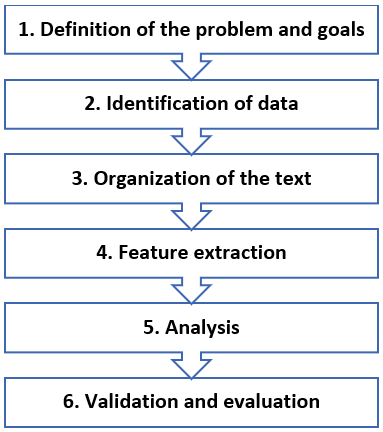
\includegraphics{images/text_mining_pipeline}
      \caption{Processing pipeline of text mining}
      \label{fig:text_mining_pipeline}
    \end{figure}
  
  \subsection{Definition of the problem and goals}
  \label{subsec:definition_of_the_problem_and_goals}
  
  \subsection{Identification of data}
  
  \subsection{Organization of the text}
  
  \subsection{Feature extraction}
  
  \subsection{Analysis}
  
    \begin{figure}[H]
      \centering
      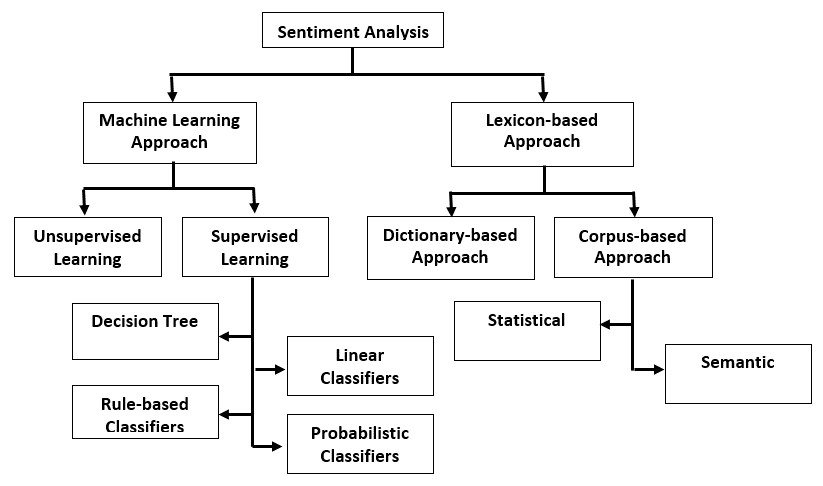
\includegraphics[scale=0.5]{images/learning_approaches_sentiment_analysis}
      \caption{Learning approaches for sentiment analysis\autocite{Halibas2018}\protect\footnotemark}
      \label{fig:learning_approaches_sentiment_analysis}
    \end{figure}
    
    \footnotetext{\url{https://www.researchgate.net/figure/Sentiment-Analysis-Source-4-Fig-1_fig1_324360275}, (11.04.2019, 23:43)}
  
    \begin{table}[H]
      \begin{tabular}{cc|c|c|c|c|l}
        \cline{3-5}
        & & \multicolumn{3}{ c| }{Predicted class} \\ \cline{3-6}
        & & a & b & c & Total \\ \cline{1-6}
        \multicolumn{1}{ |c  }{\multirow{3}{*}{Actual class} } &
        \multicolumn{1}{ |c| }{a} & 88 & 10 & 2 & 100 & \\ \cline{2-6}
        \multicolumn{1}{ |c  }{} &
        \multicolumn{1}{ |c| }{b} & 14 & 40 & 6 & 60 & \\ \cline{2-6}
        \multicolumn{1}{ |c  }{} &
        \multicolumn{1}{ |c| }{c} & 18 & 10 & 12 & 40 & \\ \cline{1-6}
        \multicolumn{1}{  c  }{} &
        \multicolumn{1}{ |c| }{Total} & 120 & 60 & 20 & 200 & \\ \cline{2-6}
      \end{tabular}      
      \begin{tabular}{cc|c|c|c|c|l}
        \cline{3-5}
        & & \multicolumn{3}{ c| }{Predicted class} \\ \cline{3-6}
        & & a & b & c & Total \\ \cline{1-6}
        \multicolumn{1}{ |c  }{\multirow{3}{*}{Actual class} } &
        \multicolumn{1}{ |c| }{a} & 60 & 30 & 10 & 100 & \\ \cline{2-6}
        \multicolumn{1}{ |c  }{} &
        \multicolumn{1}{ |c| }{b} & 36 & 18 & 6 & 60 & \\ \cline{2-6}
        \multicolumn{1}{ |c  }{} &
        \multicolumn{1}{ |c| }{c} & 24 & 12 & 4 & 40 & \\ \cline{1-6}
        \multicolumn{1}{  c  }{} &
        \multicolumn{1}{ |c| }{Total} & 120 & 60 & 20 & 200 & \\ \cline{2-6}
      \end{tabular}      
      \caption{Actual (left) and expected (right) outcomes of three-class-classification, cf.\autocite[Chapter~5.7]{Witten2005}}
      \label{tab:actual_and_expected_outcomes_of_three_class_classification}
    \end{table}  

  \subsection{Validation and evaluation}
  \label{subsec:validation_and_evaluation}
  \clearpage
  
  \section{Experimental setup}
  \label{sec:experimental_setup}
  
  \subsection{Data set extraction}
    Nur Weka-Classification oder auch ersten Ansatz der NLTK-Classification mit reinnehmen?

  \subsubsection{PGN-format}
    PGN is "Portable Game Notation", a standard designed for the representation of chess game data using ASCII text files. PGN is structured for easy reading and writing by human users and for easy parsing and generation by computer programs \autocite[Chapter~1]{Edwards1994}. A sample game in PGN notation is shown in figure~\ref{fig:sample_pgn_game}.

	\begin{figure}[H]
	  \centering
      \lstset{commentstyle=\color{blue},morecomment=[s]{\{}{\}},moredelim=[is][\bfseries]{\\textbf\{}{\}},moredelim=[is][\color{red}]{\\nag\{}{\}}}
	  \begin{lstlisting}	  
[Event "Deutschland "]
[Site "?"]
[Date "1995.??.??"]
[Round "?"]
[White "Lutz, Ch"]
[Black "Kramnik, V."]
[Result "0-1"]
[ECO "B33"]
[PlyCount "70"]
[EventDate "1995.??.??"]

\textbf{1. e4} {B33: Sicilian: Pelikan and Sveshnikov Variations} \textbf{1... c5 2. Nf3 Nc6 3.
d4 cxd4 4. Nxd4 Nf6 5. Nc3 e5 6. Ndb5 d6 7. Bg5 a6 8. Na3 b5 9. Nd5 Be7 10.
Bxf6 Bxf6 11. c3 O-O 12. Nc2 Bg5 13. a4 bxa4 14. Rxa4 a5 15. Bc4 Rb8 16. b3 Kh8
17. O-O g6 18. Qe2 Bd7 19. Rfa1 19... Bh6} {last book move} \textbf{20. g3} {
Consolidates f4} (20. Nde3 20... Be6 \nag{$14}) \textbf{20... f5} \nag{$11} \textbf{21. exf5 gxf5 22. b4
22... e4} {Black wins space.} \textbf{23. bxa5 Ne5 24. Rb4 Rxb4 25. cxb4 f4 26. Nd4 e3
27. fxe3} (27. Nxf4 \nag{$2} {doesn't work because of} 27... exf2+ 28. Qxf2 28... Bxf4
\nag{$19}) \textbf{27... f3} {He broke from his leash} (27... fxg3 28. hxg3 Qg5 29. Kh2 Nxc4
30. Nf4 \nag{$19}) \textbf{28. Qa2 f2+ 29. Kg2 Qe8 30. Be2 30... Ng4} {
The pressure on the isolated pawn grows} \textbf{31. Bf3} \nag{$4} (31. Qd2 Qh5 32. Bxg4 Qxg4
33. Nf4 Bxf4 34. exf4 Qh3+ 35. Kxf2 Qxh2+ 36. Ke1 Qxg3+ 37. Kd1 Qg1+ 38. Ke2
Bg4+ 39. Kd3 Qxa1 40. f5 \nag{$19}) \textbf{31... Nxe3+} \nag{$19} \textbf{32. Nxe3 Qxe3 33. Qxf2} \nag{$4} {
sad, but how else could White save the game?.} (33. Rd1 Bg7 34. Qb3 Bxd4 35.
Qxe3 Bxe3 36. Be2 \nag{$19}) \textbf{33... Bh3+} \nag{$1} {the final blow} \textbf{34. Kg1} {
Black now must not overlook the idea Re1} (34. Kxh3 {A deflection} 34... Qxf2)
\textbf{34... Qc3 35. Re1 Bd2} (35... Bd2 36. Ne2 36... Qxf3 \nag{$19} (36... Bxe1 \nag{$6} {
is clearly weaker} 37. Nxc3 Bxf2+ 38. Kxf2 \nag{$19}) (36... Rxf3 \nag{$2} 37. Nxc3 Rxf2
38. Kxf2 Bxc3 39. Re7 \nag{$18})) \textbf{0-1}
	  \end{lstlisting}	  

      \caption{Sample PGN game}
      \begin{tabular}{r@{: }l r@{: }l}
        blue & comments & red & NAGs
      \end{tabular}
      \label{fig:sample_pgn_game}
	\end{figure}
	
    A PGN game contains first a list of tuples with general information of the game (“tag pairs”). Seven of those tags are mandatory (Seven Tag Roster: Event, Site, Date, Round, White, Black, Result), the other tags are optional. \\\\
    Afterwards the “movetext” section starts. The chess moves themselves are represented using SAN (Standard Algebraic Notation). A move pair (one move of white and one of black) starts with the move pair number followed by a dot and a blank, then the move of white, another blank and the move of black, e.g. 
    \begin{quotation}
      7. Bg5 a6.
    \end{quotation}    
    Each move contains the piece by a single upper-case letter except of the pawn (see table~\ref{tab:basic_chess_notations}) followed by the square the piece is moved to (see figure~\ref{fig:square_names}). Hence, the example describes the seventh move of both players in the game; white moves his dark-squared bishop to the square g5 and black moves his a-file-pawn to a6. If a piece of the opponent is placed on the destination square, this piece is captured and in the move an "x" is inserted immediately before the destination square. In this case, if the capturing piece is a pawn, the lower-case letter of the previous file of the pawn is used at the beginning of the move, e.g. "exd5". Whenever a move pair is interrupted by a comment, the move of black is prefaced by the move pair number, an ellipsis and a blank: 
    \begin{quotation}
      Nxf4 \$2 \{doesn't work because of\} 27... exf2+
    \end{quotation}
    Additionally, there are some further moves with a special notation (see table~\ref{tab:basic_chess_notations}). In cases of disambiguation of pieces, an additional letter for the file or a number for the rank is used. In summary, a move can contain between two and seven signs in SAN \autocite[Chapter~8]{Edwards1994}.
	
    \begin{figure}[H]
      \begin{floatrow}
      \capbtabbox[10.4cm]{%
        \begin{tabular}{| l | l |}
    	\hline
    	Symbol & Meaning \\ \hline
    	  K & King \\ \hline
    	  Q & Queen \\ \hline
    	  R & Rook \\ \hline
    	  B & Bishop \\ \hline
    	  N & Knight \\ \hline
    	  \textit{blank} & Pawn \\ \hline
        \end{tabular}
        \begin{tabular}{| l | l | l |}
    	  \hline
    	  Symbol & Meaning & Example \\ \hline
    	  x & Capture & Rxa1 \\ \hline
    	  + & Check & Nf6+ \\ \hline
    	  \# & Checkmate & Bb7\# \\ \hline
    	  0-0 & Castling kingside & \\ \hline
    	  0-0-0 & Castling queenside & \\ \hline
    	  = & Promotion & fxg1=Q+ \\ \hline
        \end{tabular}
      }{%
        \caption{Basic chess notations}
        \label{tab:basic_chess_notations}
      }
      \ffigbox[6.6cm]{%
	    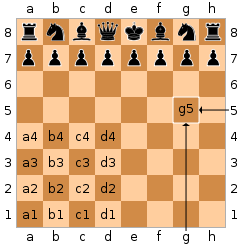
\includegraphics[scale=0.5]{images/algebraic_notation}
      }{%
	    \caption{Square names in algebraic notation\protect\footnotemark}
        \label{fig:square_names}
      }
      \end{floatrow}
    \end{figure}
    
  	\footnotetext{\url{https://en.wikipedia.org/wiki/Algebraic_notation_(chess)#/media/File:SCD_algebraic_notation.svg}, (18.03.2019, 20:56)}
  	
	Parts of the moves are annotated using comments in braces. A comment can contain information about the opening of the game, about a single move or about the current position. In the last two cases the comment is often prefaced by one or several NAGs (see below) or the corresponding chess symbol. Since there is no restriction on the exact position of a comment, comments may refer to the move before or after itself. A comment can also connect two or more moves with each other. On the contrary, a comment can be interrupted by a move such that it is split into two parts, which may only make sense when seen together. All in all, there are four possibilities of comment-move combinations shown in the examples of table~\ref{tab:comment_move_combinations}.
	
	\begin{table}[H]
      \centering
      \begin{tabular}{| l | l |}
    	\hline
    	Combination & Example \\ \hline
    	Move, Comment & e4 \{Black wins space.\} \\ \hline
    	Comment, Move & \{Weaker is\} 39. Bxe6 \\ \hline
    	Move, Comment, Move & Nxf4 \$2 \{doesn't work because of\} 27... exf2+ \\ \hline
    	Comment, Move, Comment & \{Because of the blunder\} 24. Txf8 \{Black wins immediately\} \\ \hline
      \end{tabular}      
      \caption{Comment-move combinations}
      \label{tab:comment_move_combinations}
    \end{table}
    
    Besides, by convention there should not be nested braces, however, sometimes nested braces are used to comment different move variants separately.	Those variants need not be part of a comment and are written down in parenthesis. The enumeration of the moves proceeds within a variant and is set back before a new variant starts or the game itself continues. 
   
  \subsubsection{Chessbase-DB}
  	Transformation to PGN, language detection using polyglot
  
  \subsubsection{NAGs}
	Symbols and corresponding NAGs
	
	\begin{table}[H]
      \begin{tabular}{| l | l | l |}
    	\hline
    	NAG & Symbol & Meaning \\ \hline
    	x & Capture & Rxa1 \\ \hline
    	+ & Check & Nf6+ \\ \hline
    	\# & Checkmate & Bb7\# \\ \hline
    	0-0 & Castling kingside & \\ \hline
    	0-0-0 & Castling queenside & \\ \hline
    	= & Promotion & fxg1=Q+ \\ \hline
      \end{tabular}
      \caption{Meaning of NAGs}
      \label{tab:meaning_of_nags}
	\end{table}

  \subsubsection{Python NLTK}
	RegExp parsing, tokenization, extraction of comment and class  
  
  \subsection{Prepare data for classification}

  \subsubsection{Feature extraction}
    simple features: count(word), advanced features: tf-idf, bigrams, trigrams

  \subsubsection{Generating training instances}
    structure of arff-file
	a brilliant counterattack of white
	a big mistake of black	   
    
	\begin{figure}[H]
	  \centering
      \lstset{keywordstyle=\color{blue},morekeywords={@RELATION,@ATTRIBUTE,@DATA,NUMERIC,REAL}}
	  \begin{lstlisting}
@RELATION comment
@ATTRIBUTE COUNT(brilliant) NUMERIC
@ATTRIBUTE TFIDF(mistake) REAL
@ATTRIBUTE CLASS {good,bad}
@DATA
1,0.0,good
0,0.06,bad	  
	  \end{lstlisting}	  

      \caption{Sample arff file}
      \label{fig:sample_arff_file}
	\end{figure}

	\begin{figure}[H]
	  \centering
      \lstset{keywordstyle=\color{blue},morekeywords={@DATA}}
	  \begin{lstlisting}
@DATA
{1 2, 3 good}
{2 0.06, 3 bad}	  
	  \end{lstlisting}	  

      \caption{Sample sparse arff file}
      \label{fig:sample_sparse_arff_file}
	\end{figure}
  \clearpage
  
  \section{Experiment setup}
  
  \subsection{Selecting classes}
    distribution how many instances per class, splitting into several problems: 2 classes (!,?), 6 classes (!!,!,!?,?!,?,??), 2 classes (+,-), 7 classes --> introduction of dictionary
    difference if even or odd number of classes ("neutral class")
    
  \subsection{Tokenizer tuning}
    punctuation, special chess notations (\#ce etc.)
    
  \subsection{NLTK Parameters}
    stopwords, stemming, threshold(hapax), lowercase, bigram, trigram

  \subsection{Classifiers}
    which classifier to use? --> MCC (x3), OCC, RF, NBM
  \clearpage  
  
  \section{Evaluation of results}
    tables with number of attributes, tables with accuracies, comparison of confusion matrix\\
    each for simple approach, tf-idf, word embedding
  \clearpage  
  
  \section{Conclusion}

  \subsection{Summary}

  \subsection{Outlook}
  \clearpage
  
  \paragraph{References}
  \printbibliography
  \clearpage
  
\end{document}
